% ------------------------------------------------------------------------------------
\newpage
{\color{lightgray} \hrule}
\begin{enumerate} \setcounter{enumi}{1}
	\item Simular de la distribución $Gamma(\alpha,1)$ con la propuesta $Gamma([\alpha],1)$, donde $[\alpha]$ denota la parte entera de $\alpha$. Además, realizar el siguiente experimento: poner como punto inicial $x_0 = 950$ y graficar la evolución de la cadena, es decir, $f(X_t)$ vs $t$.
\end{enumerate}

\textcolor{BrickRed}{\it Respuesta:}

En el archivo \textcolor{mediumblue}{ejercicio2\_tarea7.py} se implementa la función \textit{METROPOLIS\_HASTINGS()} la cual aplica el algoritmo Metropolis-Hastings para cualquier dimensión $n$ y toma los siguientes argumentos:
\begin{itemize}
	\item La función objetivo $f$ (en este caso es una distribución $Gamma(\alpha,1)$).
	\item La distribución propuesta $q_{gen}$ (en este caso es una distribución $Gamma([\alpha],1)$).
	\item La función $q_{pdf}$ la cual es función de densidad de probabilidad de la propuesta $q_{gen}$.
	\item El valor inicial $x_0$ (en este caso es $x_{0}=950$).
	\item El número de iteraciones del algoritmo (casi siempre se usa $N = 10,000$).
\end{itemize}

Esta función regresa la cadena de Markov simulada. Usa el criterio de aceptación: si $y_t$ es la propuesta dada por $q(\cdot|x_t)$ en $x_t$, entonces se acepta $y_t$ con probabilidad $\rho(x_t, y_t)$ con
\begin{equation}
	\rho(x,y) = \min\left\{1, \frac{f(y)}{f(x)} \frac{q(x|y)}{q(y|x)} \right\}
\end{equation}
y se rechada con probabilidad $1-\rho(x_t, y_t)$ (para este caso se utiliza $q_{pdf}$).  Se define la función objetivo \textit{f()} (que es la pdf de una distribución $Gamma(\alpha,1)$), y las funciones propuesta \textit{q\_gen()} y \textit{q\_pdf()} dada por la distribución $Gamma([\alpha],1)$. Finalmente, se simulan variables aleatorias $Gamma(\alpha, 1)$ con $3$ alphas distintos y se comparan las distribuciones obtenidas con un histograma, también se genera el gráfico que describe la evolución de la cadena. Dado que $x_0=950$ es relativamente grande, $\alpha$ no tiene que ser tan alejado de $950$ para evitar indeterminaciones y el riesgo de no converger. Para esto, se tomaron los $3$ valores de $\alpha$ tales que:
\begin{itemize}
	\item $\alpha\in[x_0-200, x_0+200]$
\end{itemize}
\begin{figure}[h!]
	\centering
	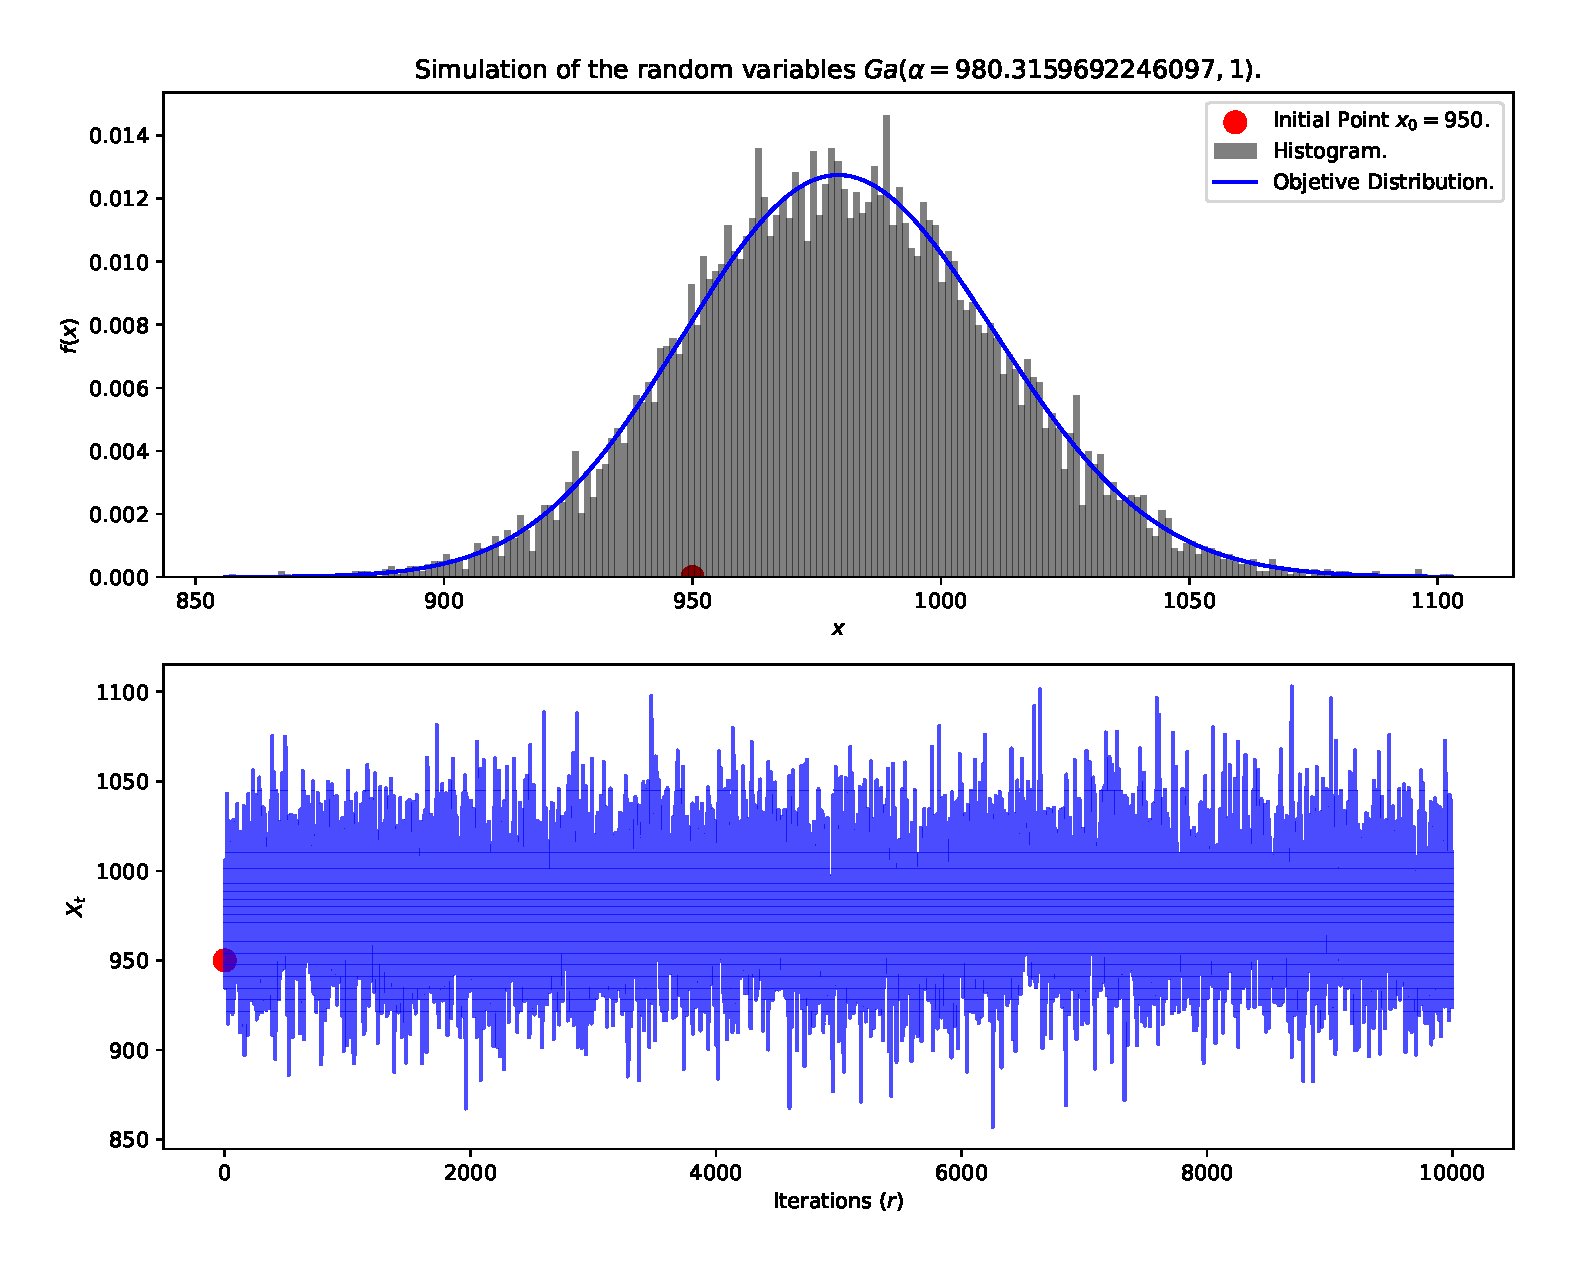
\includegraphics[width=0.6\textwidth]{IMAGENES/ex2/example1_ex2.pdf}
\end{figure}

\begin{itemize}
	\item $\alpha\in[x_0-500, x_0]$
\end{itemize}
\begin{figure}[h!]
	\centering
	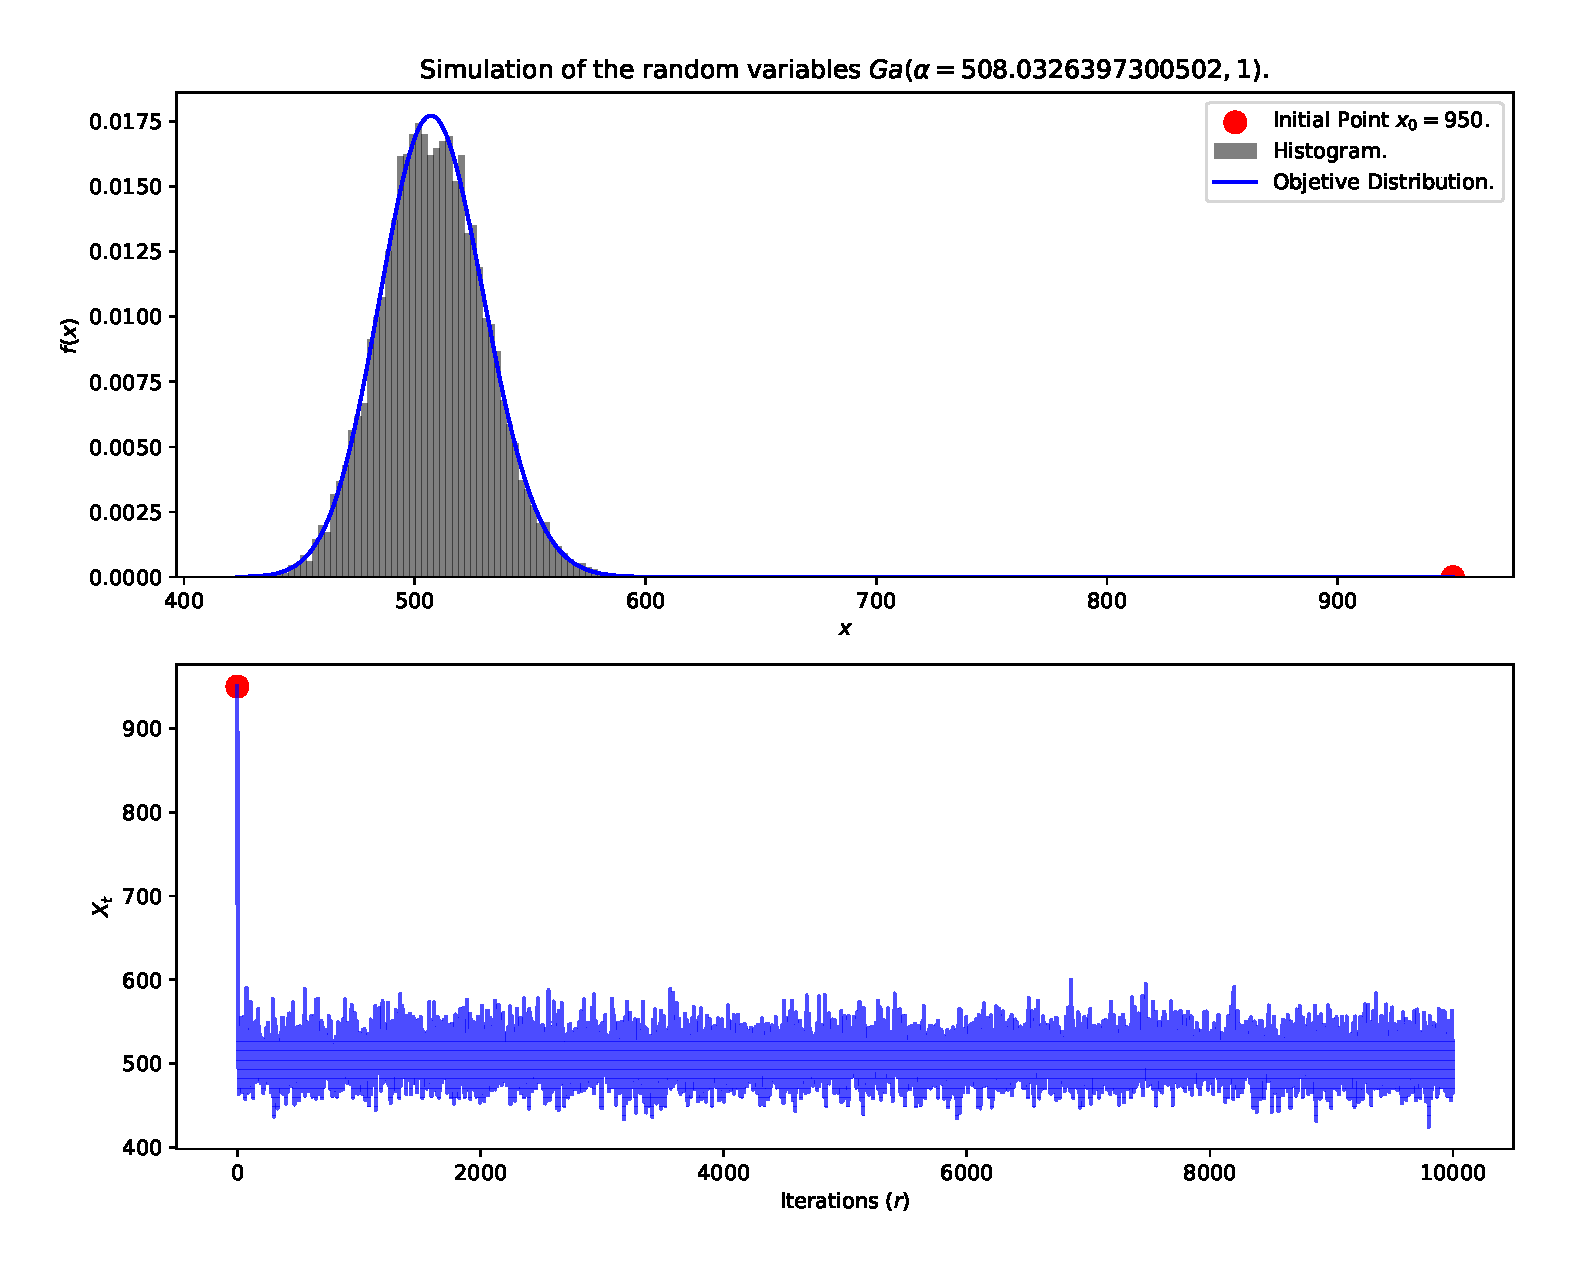
\includegraphics[width=0.6\textwidth]{IMAGENES/ex2/example2_ex2.pdf}
\end{figure}

\begin{itemize}
	\item $\alpha\in[x_0, x_0+500]$
\end{itemize}
\begin{figure}[h!]
	\centering
	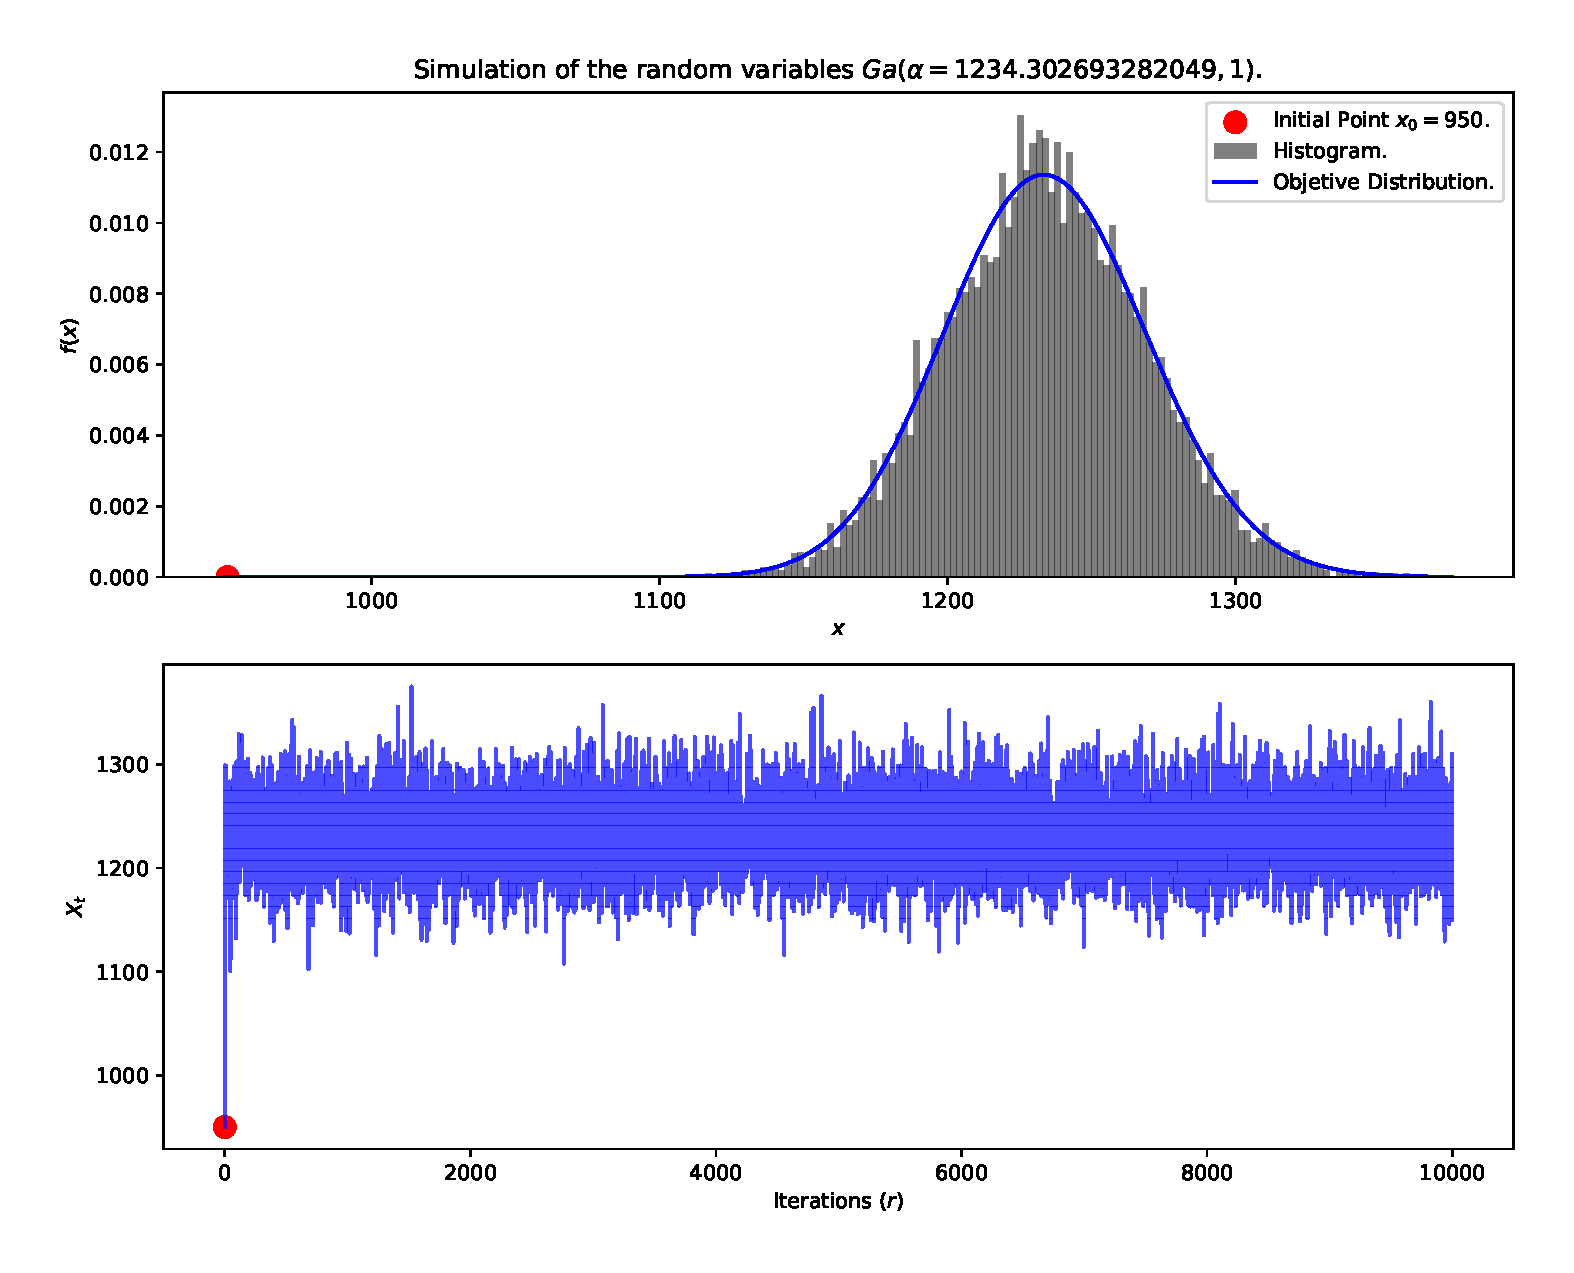
\includegraphics[width=0.6\textwidth]{IMAGENES/ex2/example3_ex2.pdf}
\end{figure}

Se simularon varios ejemplos con valores de $\alpha$ más pequeños pero, al estar tan lejos del soporte, de la distribución, tiende a generar indeterminaciones al comienzo de la cadena de Markov. Un ejemplo es el siguiente para $\alpha=10$, en donde se nota que la cadena demora un poco más en llegar a la región donde se concentra el soporte de $Gamma(10,1)$:
\begin{figure}[h!]
	\centering
	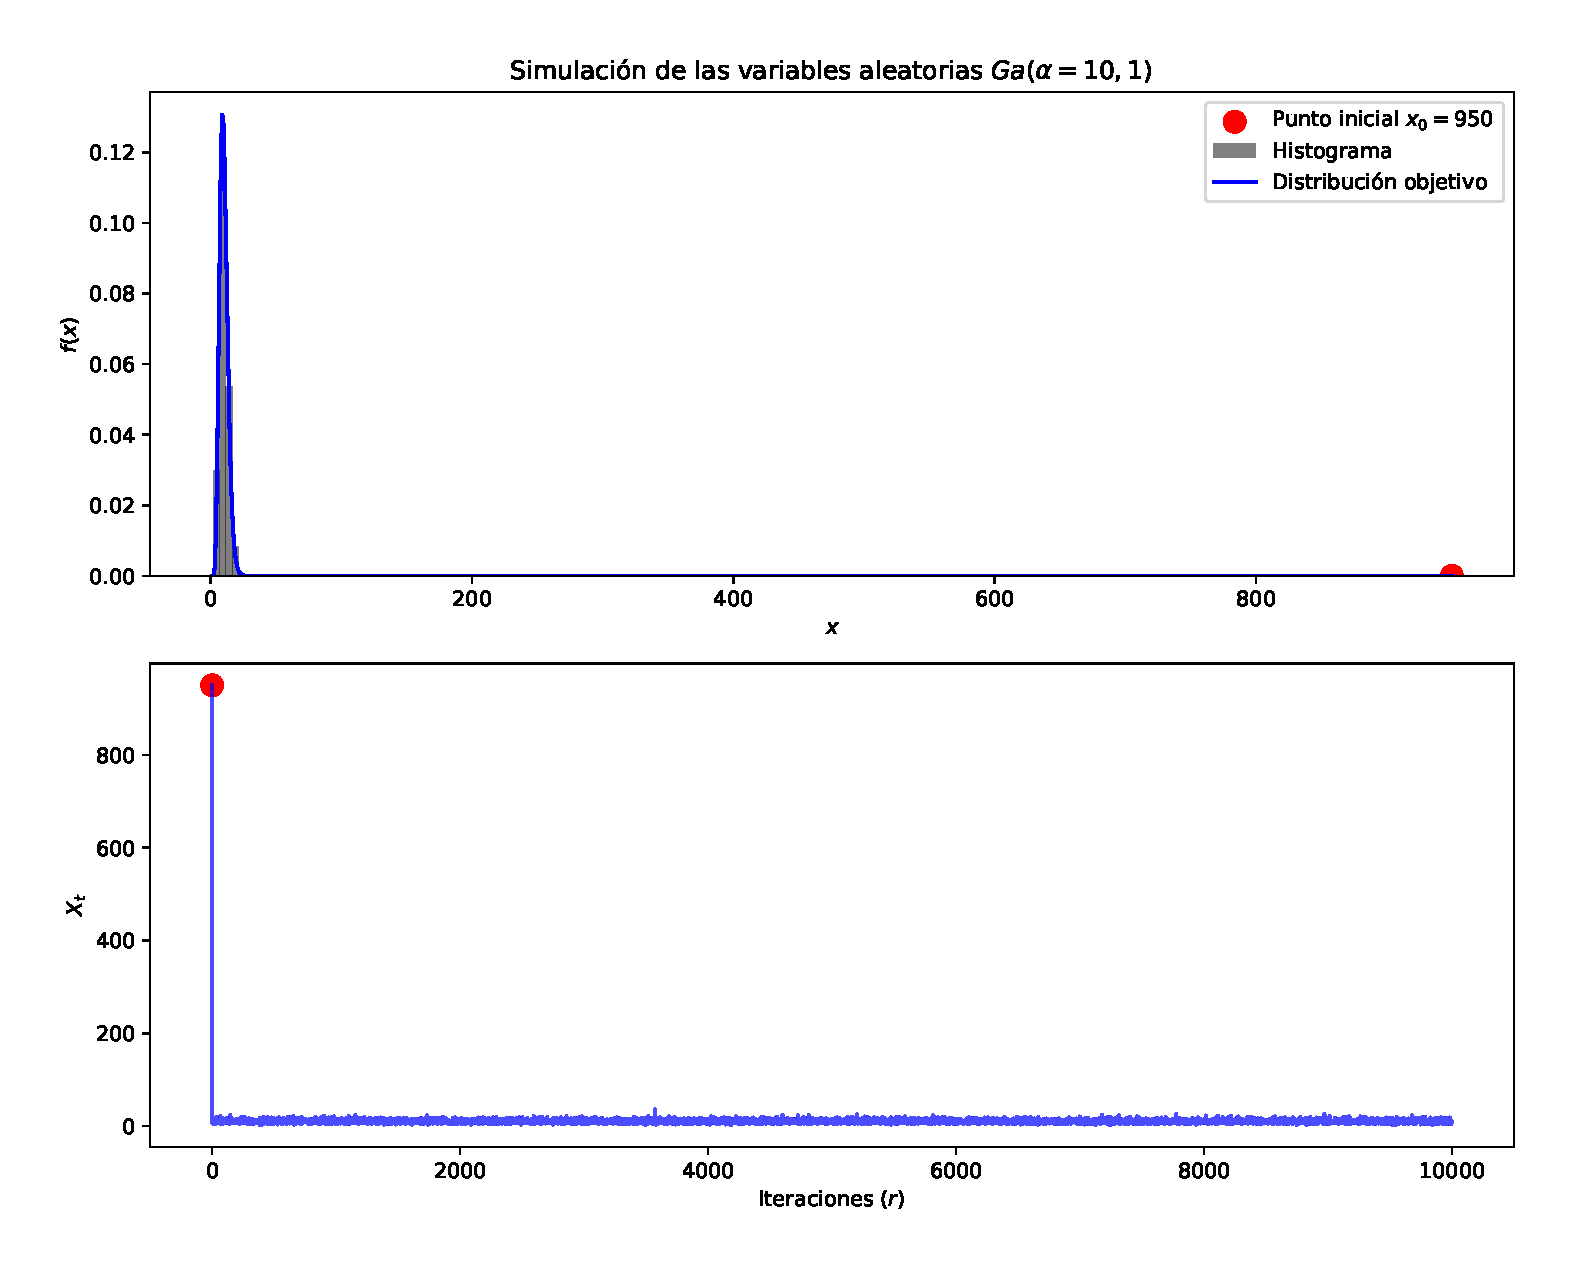
\includegraphics[width=0.8\textwidth]{IMAGENES/ejer2_alphamalo.pdf}
\end{figure}